\documentclass[addpoints, 12pt] {exam}
\usepackage{graphicx}
\usepackage{amsmath}
\bracketedpoints
\pagestyle{headandfoot}
\runningheadrule
\firstpageheader{Math 112}{Written Homework 5}{Due February 12th 2024}
\runningheader{Math 112}{ Page\; \thepage\; of\; \numpages}{Written Homework 5}
\firstpagefooter{}{}{}
\runningfooter{}{}{}
\setlength\answerskip{2ex}
\setlength\answerlinelength{1.5in}
\begin{document}

\begin{center}
\fbox{\fbox{\parbox{5.5in}{\centering
Directions:\\Please only put your final, well written solutions, in the space provided.\\ Give exact answers (simplified radicals or fractions).\\If you use additional paper clearly label the question and upload pages after the question page.\\Use complete sentences and explain your reason as much as possible.\\There are \numquestions\,  questions and \numpoints\, points total
}}}\end{center}
\vspace{0.1in}
\makebox[\textwidth]{Name:\enspace\hrulefill}
%\qformat{Question \thequestion \dotfill \thepoints}%

\begin{questions}
\question Answer each question
\begin{parts}
\part[2] If the point $(5,-3)$ is on the graph of the function $y=f(x)$, where will that point land if it is transformed by $y=\frac{2}{3}f(x-5)+1$? \vspace{1in}\answerline
\part[2] If the function $y=f(x)$ has a range of $(-1,5]$, what will the range of the transformed function $y=2f(x) -3$ be?\vspace{1in}\answerline
\part[2] Solve the equation $3x-2 = -4x +12$\vspace{1in}\answerline
\part[4] What does it mean for an equation to represent a function of $y$ in $x$?
\end{parts}\newpage
\question Consider the function given by the graph below:\newline
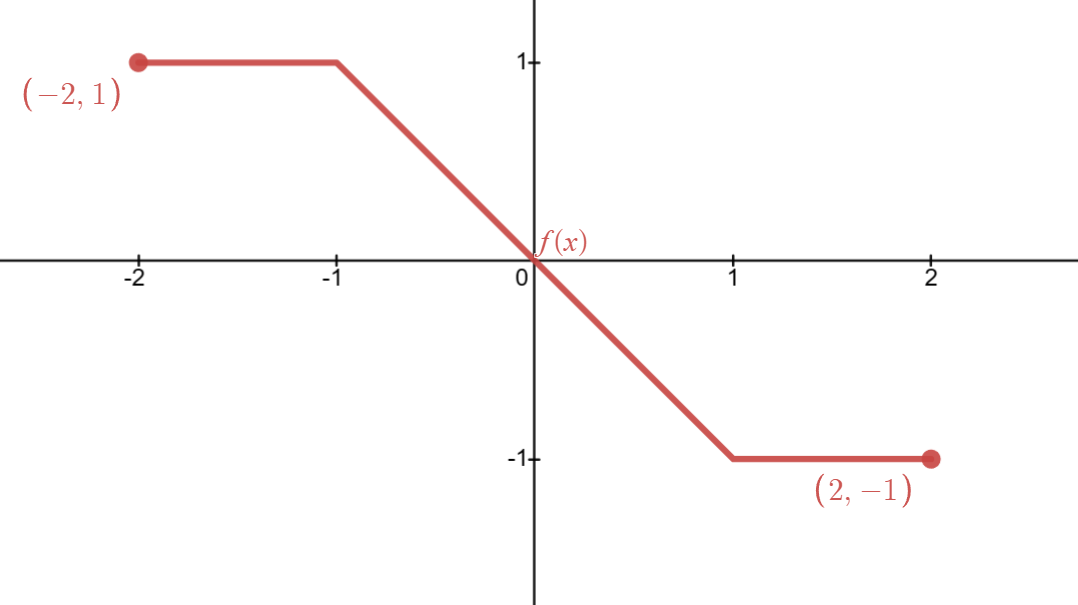
\includegraphics[scale=0.45]{piecewiselinear}\newline
\begin{parts}
\part[5] Sketch the graph of $y=2f(x-1)$. Label at least 3 of the transformed points and clearly indicate your scale. \vspace{2.5in}
\part[5] Sketch the graph of $y=-f\left(\frac{x}{2}\right)+3$. Label at least 3 of the transformed points and clearly indicate your scale. \vspace{3in}
\end{parts}
\newpage
\question Consider the function \(g(x)\) given by the graph below:\newline
\begin{center}
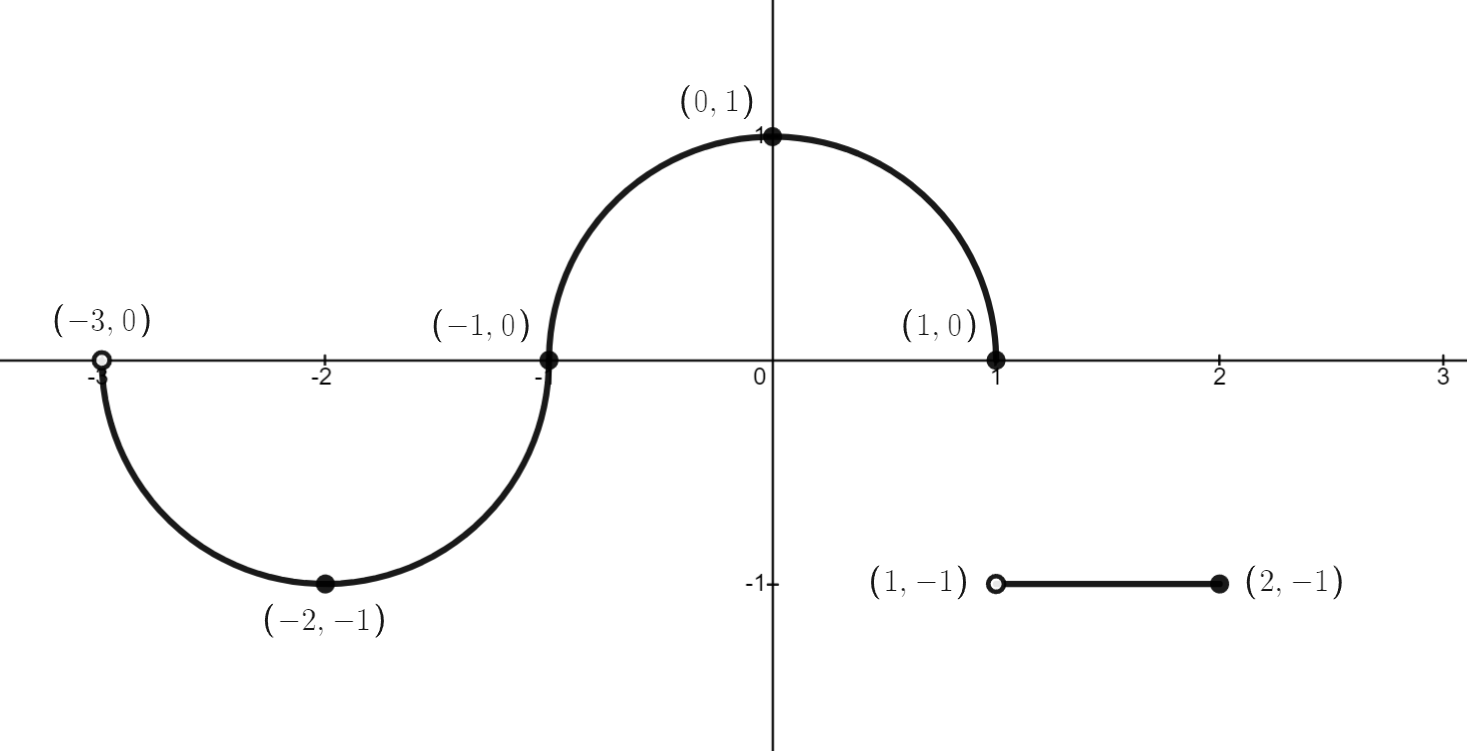
\includegraphics[scale=0.25]{transformationHW5}
\end{center}
\begin{parts}
\part[1] What is the domain of the function \(g(x)\) in the graph?\answerline
\part[1] What is the range of the function \(g(x)\) in the graph?\answerline
\part[6] Graph the transformation \(f(x) = \frac{1}{2}g(x)+2\). Include \emph{at least} 4 labeled points.\vspace{3in}
\part[1] What is the domain of the transformed function \(f(x)\)?\answerline
\part[1] What is the range of the transformed function \(f(x)\)?\answerline
\end{parts}\newpage
\question[10] \emph{Either} draw a mathematical dragon OR write a short paragraph about one. (This is intended for fun creative outlet, please put something here to receive credit)
\end{questions}


\end{document}